%%%%%%%%%%%%%%%%%%%%%%%%%%%%%%%%%%%%%%%%%%%%%%%%%%%%%%%%%%%%%%%%%
% Sirius University Presentation Template
% Author: based on Sirius University template
%%%%%%%%%%%%%%%%%%%%%%%%%%%%%%%%%%%%%%%%%%%%%%%%%%%%%%%%%%%%%%%%%

%----------------------------------------------------------
% Document Setup and Basic Packages
%----------------------------------------------------------
\documentclass[10pt]{beamer}  % Class for creating presentations, font size 10pt

% Basic packages for encoding and language support
\usepackage{cmap}             % Improves PDF search with Russian characters
\usepackage[utf8]{inputenc}   % Input encoding - UTF8
\usepackage[T2A]{fontenc}     % Support for Russian fonts
\usepackage[english]{babel}   % English language support

% Additional packages
\usepackage{animate}          % Animation support
\usepackage{upgreek}          % Upright Greek letters
\usepackage{xcolor}           % Color management
\usepackage[absolute,overlay]{textpos}  % Text positioning
\usepackage{amsmath}          % Mathematical formulas
\usepackage{fontawesome}      % Icons
\usepackage{tikz}             % Vector graphics

% Bibliography setup
\setbeamertemplate{bibliography item}{\insertbiblabel}

%----------------------------------------------------------
% Theme and Color Setup
%----------------------------------------------------------
\usetheme{default}            % Basic Beamer theme

% Define Sirius corporate color
\definecolor{Sirius}{rgb}{0.004, 0.616, 0.631} 

% Set structure elements to use the corporate color
\usecolortheme[named=Sirius]{structure}

% Add slide number to footer
\setbeamertemplate{footline}[frame number]

%----------------------------------------------------------
% Presentation Metadata Setup
%----------------------------------------------------------
\hypersetup{unicode=true}     % For correct handling of Unicode in metadata

\title[Short Title]{\bf 
Presentation Title}  % Presentation title

\date[]{}  % Date (empty by default)

\author[Author] {\bf 
Author's Full Name \\ 
Position/Title \\ 
Additional Information}

\institute[] {
Sirius University of Science and Technology \\ 
Faculty/Department Name \\ 
Laboratory/Chair Name
}

%----------------------------------------------------------
% Logo Setup
%----------------------------------------------------------
\logo{

\includegraphics[width=1.5cm]{images/Sirius-logo.png}
}

%----------------------------------------------------------
% Mathematical Commands Definition
%----------------------------------------------------------
\newcommand{\bF}{\mathbb{F}}
\newcommand{\bC}{\mathbb{C}}
\newcommand{\bP}{\mathbb{P}}
\newcommand{\bN}{\mathbb{N}}
\newcommand{\bs}{\mathbb{S}}

%----------------------------------------------------------
% Document Start
%----------------------------------------------------------
\begin{document}

%----------------------------------------------------------
% Title Slide
%----------------------------------------------------------
\maketitle

%----------------------------------------------------------
% Example Slide with Two Images
%----------------------------------------------------------
\begin{frame}{Slide Title}

\begin{figure}
    \begin{minipage}{0.45\textwidth}
        \centering
        
\includegraphics[width=\linewidth]{images/Sirius-logo.png}
        \caption{Caption for the first image}
    \end{minipage}
    \hfill
    \begin{minipage}{0.45\textwidth}
        \centering
        
\includegraphics[width=\linewidth]{images/Sirius-logo.png}
        \caption{Caption for the second image}
    \end{minipage}
\end{figure}

\end{frame}

%----------------------------------------------------------
% Example Slide with Formulas
%----------------------------------------------------------
\begin{frame}{Mathematical Formulas Example}
    \begin{equation}
        \label{eq:example}
        \begin{cases}
             \text{div}_x \bP + \boldsymbol{f} = \rho \frac{\partial^2 \boldsymbol{u}}{\partial t^2}  & \text{in domain } \mathcal{B}, \\
            \bP \cdot \boldsymbol{n} = \boldsymbol{g} & \text{on boundary } \partial \mathcal{B}_g, \\
            \boldsymbol{u} = \boldsymbol{u}_0 & \text{on boundary } \partial \mathcal{B}_u.
        \end{cases}
    \end{equation}
    
    \begin{itemize}
        \item $\displaystyle \bP = \frac{\boldsymbol{f}_{int}}{\Delta A}$ -- stress tensor
        \item Formula with reference to equation \eqref{eq:example}
    \end{itemize}
\end{frame}

%----------------------------------------------------------
% Example Slide with Bullet List
%----------------------------------------------------------
\begin{frame}{Bullet List Example}
    \begin{itemize}
        \item First list item
        \item Second list item
            \begin{itemize}
                \item Nested item
                \item Another nested item
            \end{itemize}
        \item Third list item
    \end{itemize}
\end{frame}

%----------------------------------------------------------
% Example Slide with Numbered List
%----------------------------------------------------------
\begin{frame}{Numbered List Example}
    \begin{enumerate}
        \item First step
        \item Second step
        \item Third step
    \end{enumerate}
\end{frame}

%----------------------------------------------------------
% Example Slide with Citation
%----------------------------------------------------------
\begin{frame}{Citation Example}
    Main slide content with important information.
    
    \vspace{1em}
    
    \tiny Source: Author A. et al. Article Title // Journal. – Year. – Vol. X. – P. XX-XX.
\end{frame}

%----------------------------------------------------------
% Example Slide with Full-Screen Image
%----------------------------------------------------------
\begin{frame}[plain]
    \frametitle{Full-Screen Image}
    \begin{tikzpicture}[remember picture, overlay]
        \node[at=(current page.center)] {
            
\includegraphics[width=\paperwidth,height=\paperheight,keepaspectratio]{images/Sirius-logo.png}
        };
    \end{tikzpicture}
\end{frame}

%----------------------------------------------------------
% Example Slide with Two Columns
%----------------------------------------------------------
\begin{frame}{Two Columns}
    \begin{columns}
        \begin{column}{0.48\textwidth}
            \textbf{Left Column:}
            \begin{itemize}
                \item Item 1
                \item Item 2
                \item Item 3
            \end{itemize}
        \end{column}
        \begin{column}{0.48\textwidth}
            \textbf{Right Column:}
            \begin{figure}
                \centering
                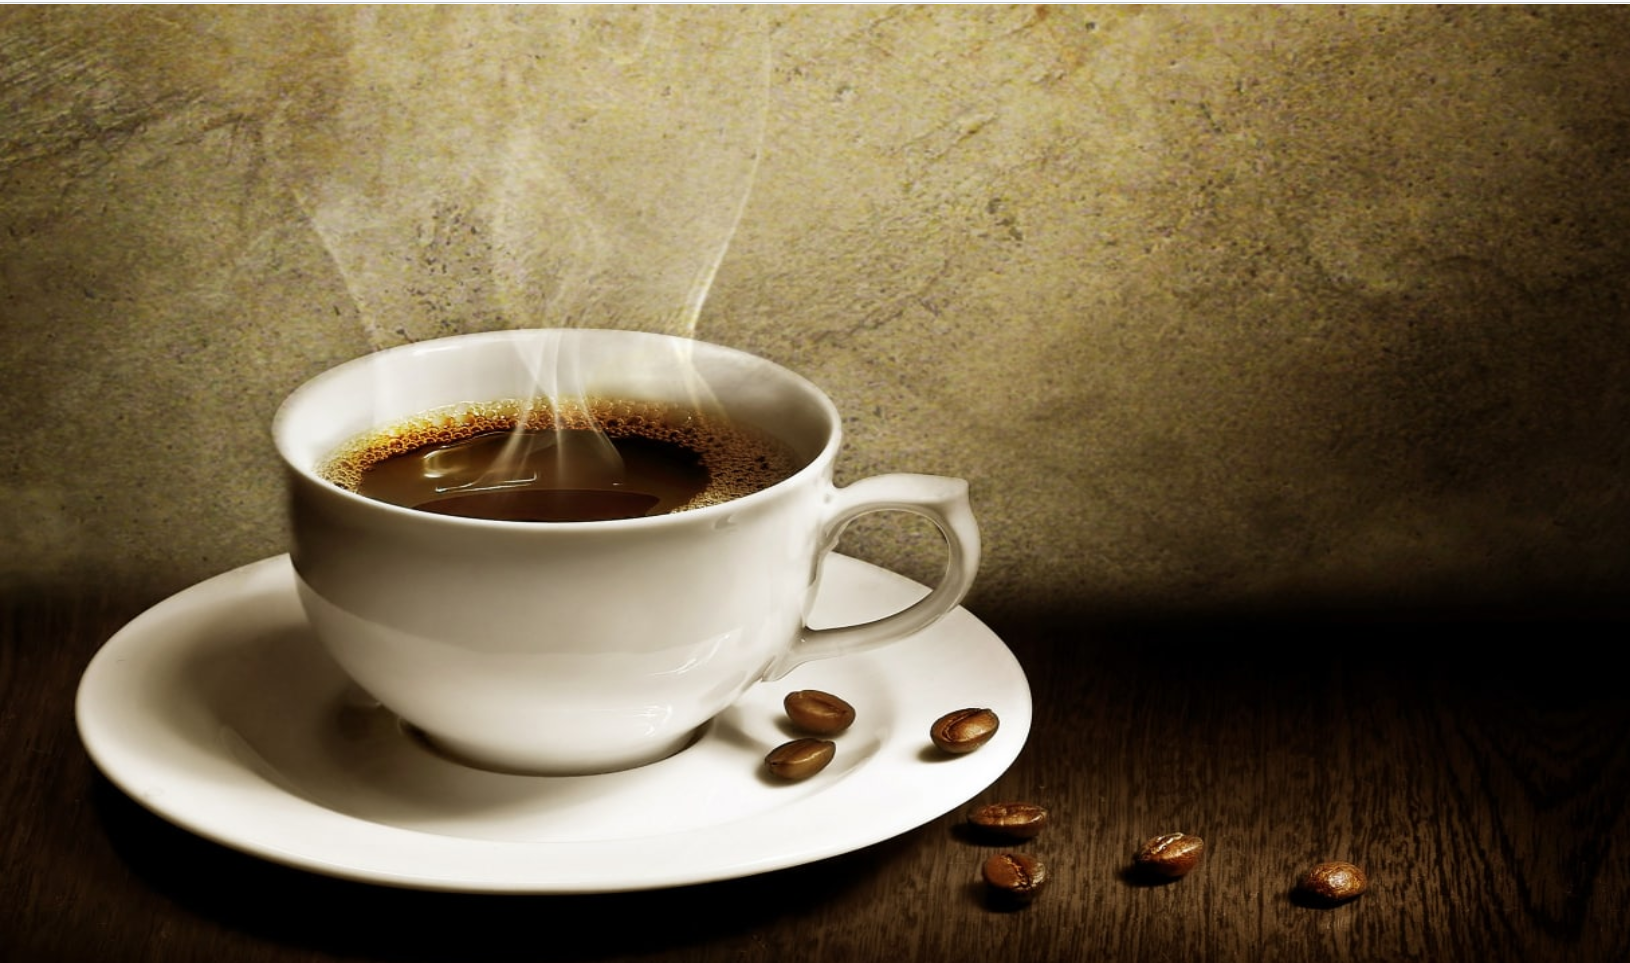
\includegraphics[width=\linewidth]{images/coffee.png}
                \caption{Image caption}
            \end{figure}
        \end{column}
    \end{columns}
\end{frame}

%----------------------------------------------------------
% Thank You Slide
%----------------------------------------------------------
\begin{frame}
    \centering
    \LARGE Thank you for your attention!
    
    \vspace{1em}
    
    \large Questions?
\end{frame}

\end{document} 